\section{BitLocker}
% https://edk2-docs.gitbook.io/edk-ii-uefi-driver-writer-s-guide/3_foundation/36_protocols_and_handles/365_tag_guid

Our final attack will target systems using BitLocker \ac{FVE} with a \ac{TPM} 2.0 and no additional PIN or startup key configured.
This leaves the Windows boot partition encrypted, the \ac{ESP} is remains unencrypted, thus not affecting the bootkit installation process.
Secure Boot can be enabled in combination of BitLocker having the effects as observed in \autoref{sec:attacks:secure-boot}, as well as additionally dictating the BitLocker default validation profile Windows uses as mentioned in \autoref{sec:windows:security:bde}.
We perform our attack against both default profiles, starting with \lstinline|{0, 2, 4, 11}|.
This means either Secure Boot is disabled or \ac{PCR}7 is not bound, because of the presence of a signature \ac{DB} other than \emph{Microsoft Windows Production PCA 2011}.
The default validation profile \lstinline|{7, 11}| used, when Secure Boot takes care of integrity validation is covered in \autoref{sec:attacks:bitlocker:bitlocker-access-without-recovery-prompt}.
Due to the boot- and rootkit still sharing their core functionality we keep the approach abstract and make no further distinctions between the two.
We refer to them with the expression \ac{UEFI} payload, not to be confused with our (Windows) payload that is deployed in the Windows installation.
For the most part of this attack we assume, that the infection is performed after BitLocker has been fully set up, only briefly touching the scenario of a user enabling BitLocker while being infected.


\subsection{Infection}

When booting with our previous \ac{UEFI} payload, the \ac{NTFS} driver is unable to recognize any file system structure  on the Windows boot partition, due to the \ac{FVE}.
Resulting in an inability to further deploy the Windows payload on the target system.
Additionally, during execution of the Windows Boot Manager, the BitLocker recovery prompt, shown in \autoref{fig:bitlocker-recovery-prompt}, interrupts the regular boot process requiring the drive's recovery key for decryption before being able to continue booting.
This happens due to \ac{TPM}'s \ac{PCR} values differing from what was initially used to seal the \ac{VMK}, leaving the Windows bootloader unable to retrieve the unencrypted \ac{VMK} from and as a result unable to decrypt the Windows installation \cite[12.]{windows-internals-7-part2}.

\begin{figure}[htb]
    \centering
    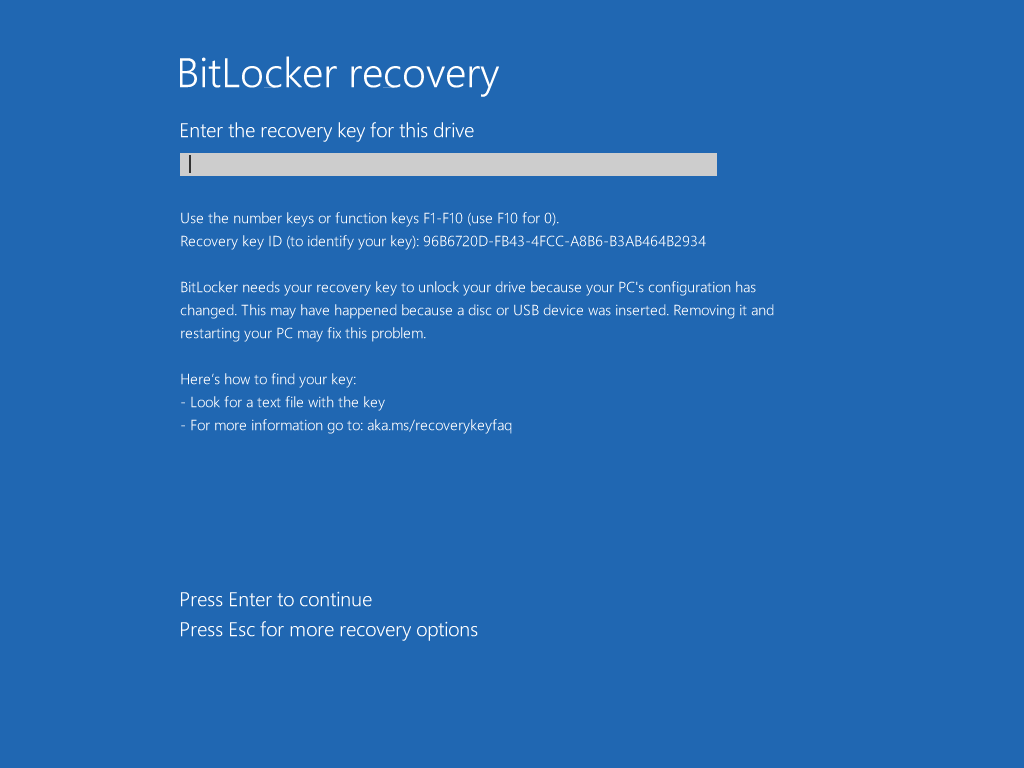
\includegraphics[width=1.0\textwidth]{attacks/bitlocker/bitlocker_recovery_prompt.png}
    \caption{BitLocker Recovery Prompt}
    \label{fig:bitlocker-recovery-prompt}
\end{figure}

BitLocker with \ac{TPM} measurements successfully mitigates \ac{UEFI} attacks and maintains system integrity by discovering deviations in the boot flow.
But how does the user react to this, after all it is asking them to enter the recovery key to resume booting and not throw out their motherboard.
There are a few options for a user to proceed, they either trust the system and enter their recovery key, mistrust the operating system or mistrust the entire system.
If they were to mistrust the \ac{OS}, or they were to have neglected to properly back up their recovery key, they might perform a fresh installation.
In the case of our bootkit this gets rid of the threat, but the rootkit remains in the firmware image and would be part of the chain of trust for the fresh installation.
If they were to mistrust the whole system, they could recover data from the drive with another system, being careful not to accidentally boot from the drive.
This would deny both our rootkit and bootkit any further access to any sensitive data.

We can look at how the user is influenced in their decision, taking a closer look at the recovery prompt in \autoref{fig:bitlocker-recovery-prompt}, we see that the message suggests a configuration change might have caused the prompt to appear. It is hinting the user that the removal of a disk or \ac{USB} stick might fix the issue (a bootable medium might change boot behavior, invalidating the \acp{PCR}). Of course this will not resolve anything in the case of an infection, but that is all the information displayed about what might have caused the issue. The rest is only about helping the user to find their recovery key to enter.
This is ground enough to argue that is very reasonable to assume that the average user will react by entering their recovery key without having any malicious behavior in mind.


\subsection{BitLogger}

When the user enters their recovery key the Windows Boot Manager uses the recovery key to decrypt the \ac{VMK} metadata entry, that was encrypted using the recovery key when BitLocker was set up.
It then proceeds to access the bitlocked \ac{NTFS} drive containing the \lstinline{Windload.efi} \ac{OS} loader.
This all still happens during the \ac{UEFI} boot environment, before \lstinline{ExitBootServices} is called.
Unfortunately we are still unable to access the Windows installation, as BitLocker only ever decrypts read operations in memory, leaving the drive fully encrypted at all times.
If we were to acquire the recovery key, we could use it to decrypt the \ac{VMK}, the \ac{FVEK} and in turn the drive ourselves.

We can achieve this by logging the keystrokes performed by a user entering the key in the recovery prompt.
Since we still are in the \ac{UEFI} boot environment, the Windows Boot Manager uses \ac{UEFI} protocols for user input instead of the own Windows drivers.
\ac{UEFI} offers two protocols for this purpose the \emph{Simple Text Input Protocol} and the \hyperref[lst:simple-text-input-ex-protocol]{Simple Text Input Ex Protocol}, we can quickly determine which of these is used by the Windows Boot manager by adding a simple \lstinline{Print} statement to the implementation in the \ac{OVMF} source code, this change also is enough to trigger the recovery prompt by invalidating the \ac{PCR} measurements.
A keystroke now shows us that the \hyperref[lst:simple-text-input-ex-protocol]{Simple Text Input Ex Protocol} is being used, the protocol structure is depicted in \autoref{lst:simple-text-input-ex-protocol}.
The Windows Boot Manager uses the \lstinline{ReadKeyStrokeEx} function to retrieve the latest pending key press.
The protocol also offers the \lstinline{WaitForKeyEx} event, signaling when keystrokes are available, execution can be blocked until this event is emitted with the \lstinline{WaitForEvent} Boot service. Example usage of the protocol can be seen in \autoref{lst:handle-protocol-simple-text-input-ex}.

\lstinputlisting[language=C,captionpos=b,label=lst:handle-protocol-simple-text-input-ex,firstline=7,caption={Example of using \emph{HandleProtocol} to retrieve an instance to the \emph{Simple Text Input Ex Protocol} to use its \emph{ReadKeyStrokeEx} function to wait for and read a pending key press}]{code/handle_protocol_simple_text_input_ex.c}

We can intercept the \lstinline{ReadKeyStrokeEx} function call by using a technique called function hooking, there are various ways of doing this, for example patching a jump instruction at the beginning of the target function to detour the execution flow.
But \ac{UEFI} protocol hooking does not require such an invasive and unportable technique.
When we take a closer look at how protocols are returned to their user we can see why.
The \ac{UEFI} Boot Services offer two functions, \lstinline{HandleProtocol} and \lstinline{OpenProtocol}, that can be used to retrieve a protocol instance. \lstinline{HandleProtocol} is a simplified abstraction of \lstinline{OpenProtocol} and is implemented by the latter internally \cite[7.3]{uefi-spec}. \lstinline{OpenProtocol} offers many additional options such as keeping track of the protocol users \cite[7.3. OpenProtocol]{uefi-spec} and exclusivity. \autoref{lst:handle-protocol-simple-text-input-ex} shows how \lstinline{HandleProtocol} can be used to receive the \hyperref[lst:simple-text-input-ex-protocol]{Simple Text Input Ex Protocol} instance installed on the active console input device \cite[4.3. EFI System Table]{uefi-spec}.
The input parameters are a device handle, the \ac{GUID} identifying the protocol and the address of a pointer to the protocol structure.
When calling \lstinline{HandleProtocol} the value of the pointer is modified to point to the corresponding protocol instance.
The protocol instance itself is previously allocated by a driver and installed onto the device handle in their Driver Binding Start function \TODO{Driver binding}.
The driver assigns the function fields with functions residing in the driver's image.
This is why it is important for a driver's image to remain loaded even after initial execution.
The important fact about this process is, that a driver installs only one protocol instance per device handle and every protocol user receives the same address for to the same protocol instance, given they use the same device handle.
The function interfaces of \lstinline{HandleProtocol} and \lstinline{OpenProtocol} would generally allow for the return of allocated memory containing a copy of the protocol's content, but the implementors of drivers managing multiple devices are encouraged to keep track of private data, that is necessary to manage a device, but not part of the protocol interface. This private data struct contains the protocol instance, so that it is then possible to calculate the private data address using the protocol instance's address and the offset of the protocol within the struct \cite[8]{tianocore-edk2-driver-writer-s-guide}. In \autoref{lst:private-data} we show an example of retrieving private data through the public protocol interface. This keeps the protocol interface clean and limited to the public functionality, but the \ac{UEFI} boot services don't know about the size of the private data when managing protocol instances and therefor cannot make copies spanning the entire data. On top of that, private data likely contains information about the device state, changes in the state would have to occur in all instances of each protocol user instead, this would defeat the concept of private data.

\lstinputlisting[language=C,captionpos=b,label=lst:private-data,firstline=6,caption={Example of a driver using private data in the implementation of the \emph{Disk I/O Protocol} \cite[8.2 and 8.5]{tianocore-edk2-driver-writer-s-guide}}]{code/private_data.c}

Since our \ac{UEFI} payload is executed before the Windows Boot Manager we can query all instances of the \hyperref[lst:simple-text-input-ex-protocol]{Simple Text Input Ex Protocol} and change the function pointer of \lstinline{ReadKeyStrokeEx} to point to our function hook.
When a user later receives a pointer to the protocol instance, accessing the \lstinline{ReadKeyStrokeEx} field will cause our hook to be called instead of the original function.
The hook has to be implemented in a driver, so that it remains loaded until the Windows Boot Manager uses \lstinline{ReadKeyStrokeEx}.
We also have to save the original function address, together with a pointer to the protocol instance, so that we can call it later.
Multiple different drivers could offer the same protocol, resulting in different functions being called depending on the device, the protocol instance is retrieved from.
When our hook is called we start by identifying which original function needs to be called using the protocol instance that is used as the first argument of the \lstinline{ReadKeyStrokeEx} function signature.
We then call the original to read the pending keystroke, keeping track of the keystrokes (separately for each protocol instance), before returning the key data back to the caller.
We coin this BitLocker specific keylogger \emph{BitLogger}. A simplified version of how the hooking process works can be seen in \autoref{lst:hooking};

\lstinputlisting[language=C,captionpos=b,label=lst:hooking,firstline=4,caption={Simplified example of hooking the \emph{Simple Text Input Ex Protocol}}]{code/hooking.c}

We want to use the recovery key programmatically, so we can't simply log all key presses in chronological order and evaluate them by hand later.
The BitLocker recovery prompt has a few rules and does not allow the user to just input any possible combination of digits, each entered block is checked for validity before allowing the cursor to advance to another block, this also applies when moving the cursor backwards to a previously entered block, while incomplete blocks are not evaluated.
Each block must be divisible by 11 \cite[9. BitLocker Key Recovery]{windows-internals-6-part2}.
For this reason and because the cursor can be used to increment and decrement the current digit by using the up and down arrow keys, we have to implement internal tracking of the cursor advancement.
The recovery prompt in \autoref{fig:bitlocker-recovery-prompt} also tells us, that the function keys (F1-F10) are accepted as input, with F10 mapping to zero, so we have to log these key presses as well.

\subsection{Dislocker}

To make use of the recovery key we can use an open source software called \emph{Dislocker}, which implements the \ac{FUSE} interface to offer mounting of BitLocker encrypted partitions under Linux supporting read and write access \cite{dislocker}.

In \autoref{sec:windows:security:bde} we discussed, how the BitLocker filter driver integrates into the Windows.
To integrate Dislocker into \ac{UEFI} start by analyzing how the \ac{NTFS} driver works.
We can start by checking the \lstinline{.inf} file of the driver, which declares which protocol \acp{GUID} are consumed and produced by the driver. \autoref{lst:uefi-driver}

\lstinputlisting[language=C,captionpos=b,label=lst:uefi-driver,caption={Protocols section of \ac{NTFS} driver's module file}]{code/uef_driver.inf}

We can ignore the last three protocols as they are not directly involved in media access.
The \hyperref[lst:simple-filesystem-protocol]{Simple File System Protocol} is produced by the driver, as it installs the protocol onto handles of devices it supports.
So the only relevant protocols it consumes are the \emph{Disk \ac{I/O} Protocol} and the \emph{Block \ac{I/O} Protocol} as well as their respective asynchronous counterparts marked by the trailing 2.
We will ignore the asynchronous protocols, as they only serve to further abstract their synchronous version \cite[13.8 and 13.10]{uefi-spec}.
The same could be said for the \emph{Disk \ac{I/O} Protocol}, as it abstract the \emph{Block \ac{I/O} Protocol} to offer an offset-length driven continous access to the underlying block device \cite[13.7]{uefi-spec}, but this is the protocol primarily used by the driver and the \emph{Block \ac{I/O} Protocol} is only used directly to retrieve volume and block size, as well as read the first block to determine whether the volume is \ac{NTFS} formatted.
Keeping in mind the fact, that the \hyperref[lst:simple-filesystem-protocol]{Simple File System Protocol} is only used to open a volume and any further access to the volume is done through the \hyperref[lst:file-protocol]{File Protocol}.
It becomes obvious that all file-wise operations are, is multiple layers of abstraction on top of block-wise access to the underlying media, performed through the \emph{Block \ac{I/O} Protocol}.
Inspired by the BitLocker filter driver in \autoref{fig:bitlocker-volume-access-driver-stack}, which de- and encrypts each block as it passes through, we hook the \emph{Block \ac{I/O} Protocol} functions \lstinline{ReadBlocks} and \lstinline{WriteBlocks}, their signatures are shown in \autoref{lst:block-io-protocol}.
We can then use Dislocker on read and write operations to implement our own filter driver as shown in \autoref{fig:dislocker-volume-access-protocol-stack}.


\begin{figure}[htb]%
    \centering
    \includesvg{dislocker_volume_access_protocol_stack.drawio.svg}
    \caption{Dislocker Volume Access Protocol Stack}%
    \label{fig:dislocker-volume-access-protocol-stack}%
\end{figure}

When we look at the Dislocker source code, we find that Dislocker works with two main functions \lstinline{dislock} and \lstinline{enlock}, they each take offset-length paremeters, comparable to the \emph{Disk \ac{I/O} Protocol} abstraction.
\lstinline{dislock} reads and decrypts, while \lstinline{enlock} encrypts and writes.
Internally Dislocker uses \lstinline{pread} and \lstinline{pwrite} to access the volume.
These operations are always performed on whole blocks, as BitLocker encryption is done block-wise.
So the starting offset is rounded down and the offset plus length is rounded up the to next block boundary.
We can map \lstinline{pread} and \lstinline{pwrite} to call the original \lstinline{ReadBlocks} and \lstinline{WriteBlocks} functions.
Since the two Dislocker functions expect offset-length, we simply multiply the starting block index by the block size to use as starting offset.


% execute after NTFS driver by doing it in an ExitBootServices hook
For the previous two attacks the timing of deploying the payload did not matter, as long as it was done before Windows loads the \lstinline{HKLM\SOFTWARE} registry hive, thus performing the deployment as soon as the \ac{UEFI} payload is executed suffices, as this happens before any Windows boot related actions are performed.
With BitLocker we have to deploy after our BitLogger was able to obtain the recovery key.
After initializing Dislocker with the recovery key we enable the transparent \emph{Block \ac{I/O} Protocol} hook layer, so we can trigger the \ac{NTFS} driver to (re-)evaluate which device handles it supports.
The BitLocker encrypted drive now appearing unencrypted allows the driver to install its \hyperref[lst:simple-filesystem-protocol]{Simple File System Protocol} instance.
This allows us to deploy the payload and import our modified registry key.
After doing this we need to disable the Dislocker layer again, as otherwise Windows is unable to boot and instead attempts Windows recovery, showing a second recovery prompt, but now outside the \ac{UEFI} environment with their own device drivers.
This recovery environment is located on the unencrypted \ac{NTFS} partition created during installation and also accessible when pressing the escape key during the initial \ac{UEFI} environment recovery prompt.
We want to prevent the user from using this prompt instead of the \ac{UEFI} prompt, as our \emph{BitLogger} would not be able to obtain the recovery key.
This can be done in our \lstinline{ReadKeyStrokeEx} hook, where when a user presses escape we instead return another key to the Windows Boot Manager.

% only necessary because the way dislocker currently checks whether the recovery key is correct is slow and impacts the user experience during recovery prompt
\TODO{if we want we can explain this}
\cite{exitbootservices-hooking}
hook ExitBootServices
enable hook
write payload
import registry key
disable hook


% finally update TPM values
If we were to attack Windows 10 we would be done now, but Windows 11 will show the recovery prompt every boot.
Windows 10 seems to automatically reseal the \ac{VMK}, whereas Windows 11 doesn't, so our \ac{UEFI} payload keeps invalidating the \ac{PCR} values.
We can add a few calls to the BitLocker management tool \lstinline{manage-bde} \cite{microsoft-bitlocker-manage-bde} within our Windows payload, deleting the old \ac{TPM} protector and adding a new one.
Now our \ac{UEFI} payload is part of the measurements and considered trusted.
Execution does not trigger the BitLocker recovery prompt anymore.

\subsection{BitLocker Access without Recovery Prompt}
\label{sec:attacks:bitlocker:bitlocker-access-without-recovery-prompt}

When either the BitLocker validation profile is misconfigured (for example \lstinline|{7, 11}|) or the \ac{TPM} protector already includes our \ac{UEFI} payload in its \ac{PCR} measurements, the \ac{TPM} yields the Windows Boot Manager the unencrypted \ac{VMK} with which it is able access the drive.
We are unable to receive a recovery key as none has to be entered and in turn we cannot decrypt the drive.
In the case of our own \ac{TPM} protector update, we could simply save the recovery key in an unencrypted region of the drive, but there is a solution which does not require any prior knowledge about the recovery key.

hook \ac{TCG}2 Protocol \cite[6.7.3]{tcg-efi-protocol-spec}
\ac{TPM} communication
% \cite[12.7 \lstinline{TPM_Unseal}]{tcg-tpm-library-part3-commands}
receive bitlocker \ac{VMK} key and send to dislocker
\cite{bde-format-spec}
\cite{tpm-sniffing}
% https://labs.withsecure.com/publications/sniff-there-leaks-my-bitlocker-key

This increases the persistence and applicability of our attack immensely.